\documentclass[10 pt,usenames,dvipsnames, oneside]{article}
\usepackage{../../../modelo-ensino-medio}



\begin{document}

\begin{center}
  \begin{minipage}[l]{3cm}

\includegraphics[width=2cm]{logo}    
\end{minipage}\hfill
\begin{minipage}[r]{.8\textwidth}
 {\Large \scshape Atividade: Quadros na parede}  
\end{minipage}
\end{center}
\vspace{.2cm}

\ifdefined\prof
\begin{objetivos}
\item \phantom{a}
\end{objetivos}

\begin{goals}
\begin{enumerate}
\item Introduzir o conceito de Progressão Aritmética.
\item  Fazer medições e criar estratégias para resolver um problema prático.
\item  Obter uma expressão que relacione a distância do gancho até a lateral da parede com o número do gancho.

\end{enumerate}

\tcblower

\begin{itemize}
\item Compartilhe com a turma algumas das soluções encontradas. Estimule que os estudantes descrevam suas estratégias e critiquem o raciocínio uns dos outros.
\item  Considere escrever um resumo dos valores bem-sucedidos no quadro, em
forma de lista.
\item  Não é exigido que os quadros sejam distribuídos de modo que as distâncias do primeiro e último quadros até as paredes laterais sejam iguais. Ou seja, os ganchos podem ser dispostos de modo que o conjunto de quadros fique mais próximo da parede da esquerda ou da direita.
\end{itemize}

\end{goals}

\bigskip
\begin{center}
{\large \scshape Atividade}
\end{center}
\fi

Caso tenha disponibilidade, sugerimos o uso da versão digital desta atividade disponível neste \href{https://teacher.desmos.com/activitybuilder/custom/5e7ba1a876309d7f9879af12}{link}

\begin{figure}[H]
\centering

\includegraphics[width=100bp]{qr_code_quadros}

\end{figure}

Você deseja pedurar três quadros que têm as mesmas dimensões na parede acima do seu sofá. A linha tracejada da figura indica a altura que você deve pedurar os ganhchos. Sem auxílio de instrumentos de medição marque as posições aproximadas dos ganchos sobre a linha tracejada de maneira que os quadros fiquem igualmente espaçados entre si.

\begin{figure}[H]
\centering
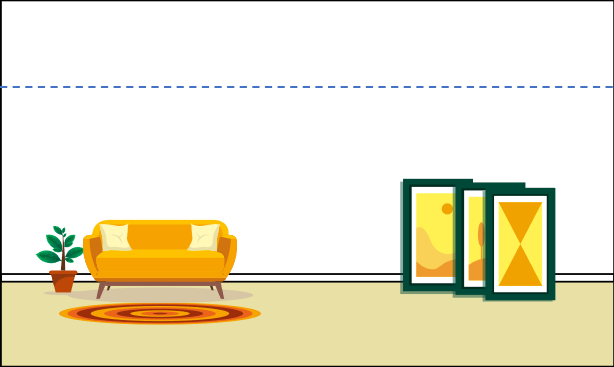
\includegraphics[width=300bp]{quadros_na_parede1}

\caption{Fonte: \href{freepik.com}{Freepik}}

\end{figure}

\begin{enumerate}
\item Marcar as posições "de olho"{}pode gerar imprecisões. Para que fique perfeito é necessário medir e distribuir uniformemente os ganchos. Com o auxílio de uma régua meça a parece acima ($1$cm=$1$m) e marque as posições para os três ganchos de pendurar quadros, precisamente. Use uma caneta de outra cor para comparar com as posições anteriores. Explique sua estratégia.

\item Agora, suponha que você tem uma outra parede representada abaixo em que deseja pendurar cinco quadros equidistantes. Onde você deve posicionar os ganchos? Use o desenho abaixo para indicar e explique a sua estratégia.

\begin{figure}[H]
\centering
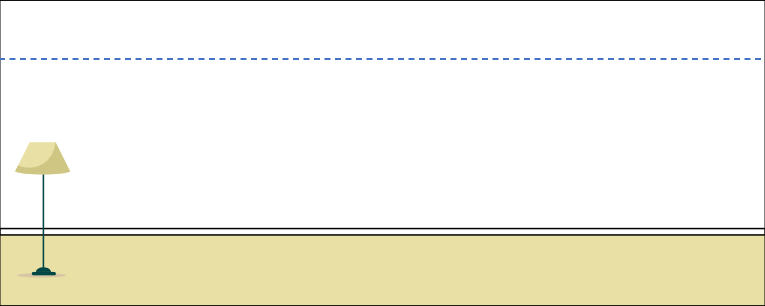
\includegraphics[width=300bp]{quadros_na_parede2}


\end{figure}

\item A tabela a seguir indica duas das distâncias (até o lado esquerdo da parede) de ganchos equidistantes em uma parede. Complete os espaços em branco e explique sua estratégia.

\begin{table}[H]
\centering
\begin{tabu} to \textwidth{|c|c|}
\hline
\thead
Gancho & Distância (m) \\
\hline
1 & \\
\hline
2 & 11 \\
\hline
3 & \\
\hline
4 & \\
\hline
5 & 23 \\
\hline
\end{tabu}
\end{table}

\item Supona agora que você queira posicionar mais 15 quadros na parede do item anterior, respeitando as distâncias estabelecidas. Como saber a distância, até o lado esquerdo da parede, que se encontra o gancho de número 10? Descreva pelo menos duas estratégias diferentes.

\item Para a parede do item anterior, escreva uma expressão que forneça a distância $d$ dos ganchos até o lado esquerdo da parede em função do número $n$ do gancho.

\item Em uma outra parede a distância dos ganchos \textit{em metros} em função da sua posição é dada por $d(n)=3+2n$. A que distância está o primeiro gancho? E o sexto gancho? O que representa o número $d(13)$?

\item Júlia e Camila usaram as seguintes expressões para representar a tabela a seguir:

\begin{table}[H]
\centering
\begin{tabu} to \textwidth{l>{$}l<{$}}
\text{Júlia} & d(n)=7+3n \\
\text{Camila} & d(n)=10+3(n-1)
\end{tabu}
\end{table}

\begin{table}[H]
\centering
\begin{tabu} to \textwidth{|c|c|}
\hline
\thead
Gancho & Distância (m) \\
\hline
1 & 10 \\
\hline
2 & 13 \\
\hline
3 & 16 \\
\hline
4 & 19 \\
\hline
5 & 22 \\
\hline
6 & 25 \\ 
\hline
\end{tabu}
\end{table}

Quem das duas se expressou corretamente? Por quê? Como cada uma delas pode ter pensado para chegar nas expressões?

\end{enumerate}

\ifdefined\prof
\begin{solucao}
\begin{enumerate}

\item Resposta individual;
\item Resposta individual;
\item Os valores que estão faltando são, nesta ordem, $7$, $15$ e $19$.
\item Uma possibilidade é desenvolver a sequência até o décimo termo que é $43$. Outra possibilidade é utilizar uma expressão que relacione a distância com o número n que indica a posição do quadro na parede, como por exemplo $d(n)=7+4(n-1)$.
\item $d(n)=7+4(n-1).$
\item $d(1)=5m$, $d(6)=15m$, $d(13)$ representa a distância do gancho $13$ até a parede.
\item Ambas se expressaram corretamente, uma vez que as expressões são equivalentes, isto é, $d(n)=10+3(n-1)=7+3n$. 

\end{enumerate}
\end{solucao}
\fi

\end{document}